\documentclass[tikz, border=50pt]{standalone}

\usepackage{tikz}
\usepackage{medl_colors}
\usepackage{amsmath,xstring}
\usepackage{ifthen}
\usepackage{geometry}
\usepackage{graphicx}

\usetikzlibrary{shapes.multipart, shapes.geometric, arrows.meta, decorations.pathreplacing, calligraphy}
\usetikzlibrary{matrix, calc, positioning,fit, backgrounds,3d}  

\graphicspath{ {./images/} }

\def\outputs{{0,1000,999,2,1}}

\begin {document}
\begin{tikzpicture}

\newcommand\cube[7]
{
\filldraw[#7] (#1+#4,#2,#3) -- (#1+#4,#2+#5,#3) -- (#1,#2+#5,#3) -- (#1,#2,#3) -- cycle;
\filldraw[#7] (#1+#4,#2,#3) -- (#1+#4,#2,#3+#6) -- (#1+#4,#2+#5,#3+#6) -- (#1+#4,#2+#5,#3) -- cycle;
\filldraw[#7] (#1+#4,#2+#5,#3) -- (#1,#2+#5,#3) -- (#1,#2+#5,#3+#6) -- (#1+#4,#2+#5,#3+#6) -- cycle;
}

\node[canvas is zy plane at x=0,draw,fill=white] (inputpic) at (-2,3,-3) {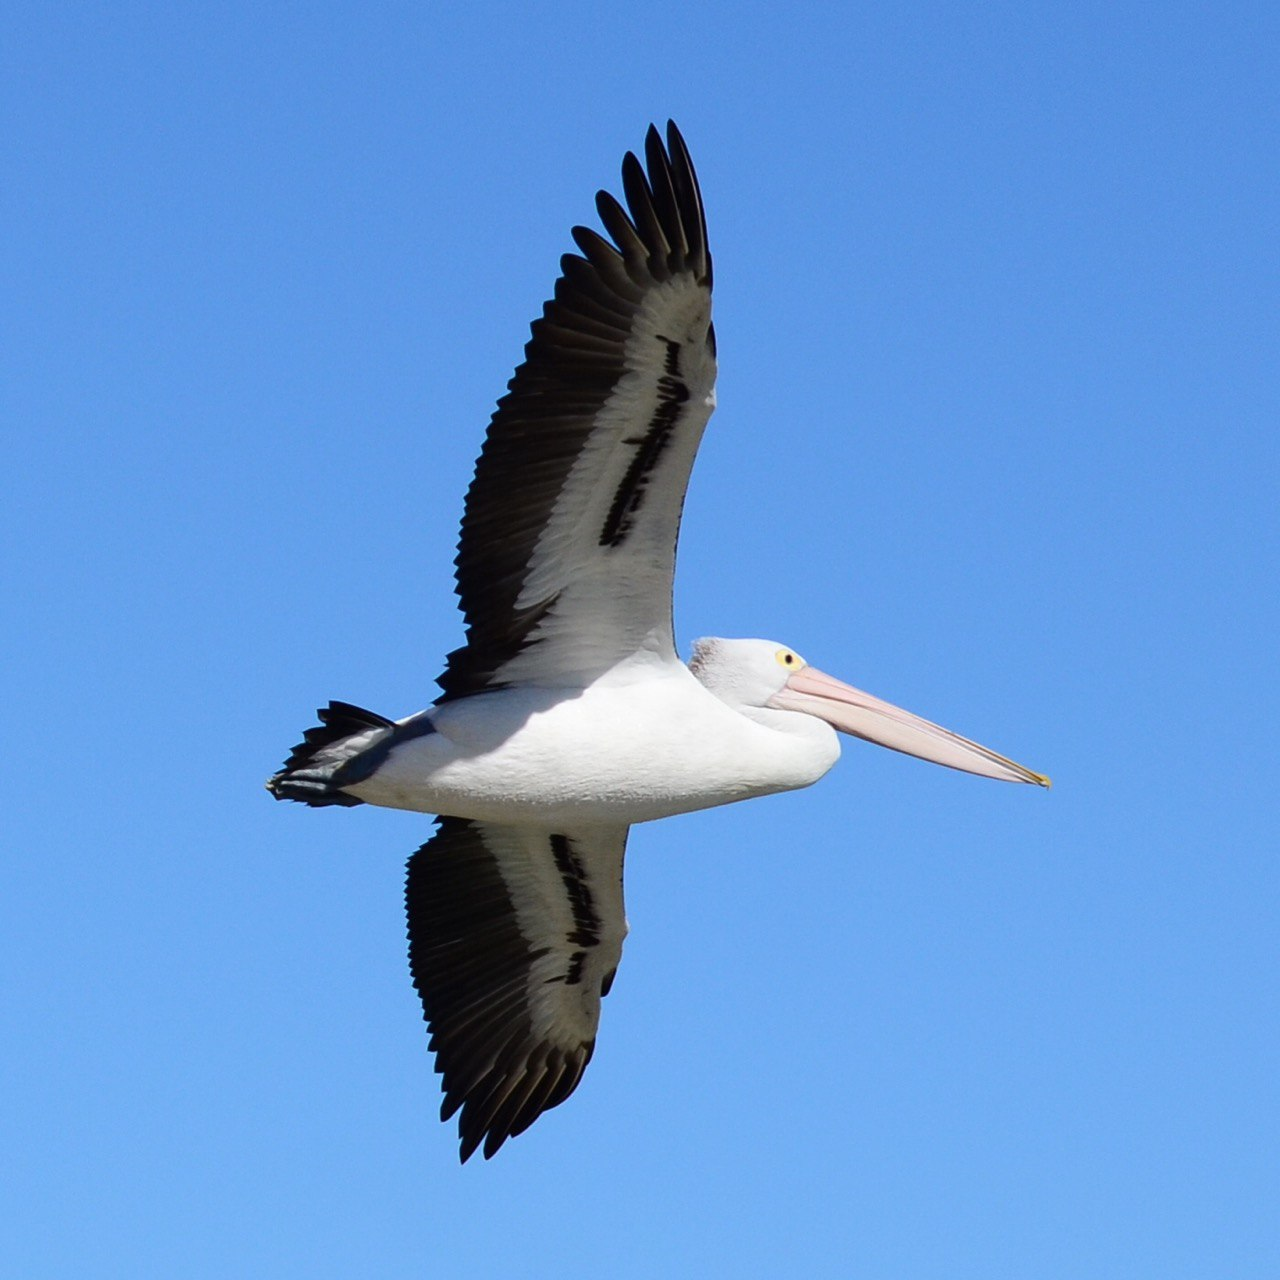
\includegraphics[scale=.14]{images/bird.jpeg}};

\cube{0}{0}{0}{.2}{6}{-6}{blueshape}
\cube{.5}{0}{0}{.2}{6}{-6}{blueshape}

\cube{1.5}{1}{1}{.2}{5}{-5}{greenshape}
\cube{1.9}{1}{1}{.4}{5}{-5}{blueshape}
\cube{2.5}{1}{1}{.4}{5}{-5}{blueshape}

\cube{3}{1.5}{.5}{.4}{4}{-4}{greenshape}
\cube{3.7}{1.5}{.5}{.6}{4}{-4}{blueshape}
\cube{4.6}{1.5}{.5}{.6}{4}{-4}{blueshape}
\cube{5.4}{1.5}{.5}{.6}{4}{-4}{blueshape}
\cube{6.2}{1.5}{.5}{.6}{4}{-4}{blueshape}

\cube{7}{2.1}{.5}{.6}{3}{-3}{greenshape}
\cube{7.9}{2.1}{.5}{.8}{3}{-3}{blueshape}
\cube{9}{2.1}{.5}{.8}{3}{-3}{blueshape}
\cube{10}{2.1}{.5}{.8}{3}{-3}{blueshape}
\cube{11}{2.1}{.5}{.8}{3}{-3}{blueshape}

\cube{12}{2.7}{.5}{.8}{2}{-2}{greenshape}
\cube{13}{2.7}{.5}{.8}{2}{-2}{blueshape}
\cube{14}{2.7}{.5}{.8}{2}{-2}{blueshape}
\cube{15}{2.7}{.5}{.8}{2}{-2}{blueshape}
\cube{16}{2.7}{.5}{.8}{2}{-2}{blueshape}
\cube{17}{3.3}{.5}{.8}{1}{-1.3}{greenshape}

\node[style={yslant=0.9,xslant=0}] at (-3,-2,-6) { \Huge $x$ };

\node[] (first) at (-1.5,8,-3) {\Large $3 \times 224 \times 224$};

\draw[decorate, decoration={calligraphic brace,amplitude=5pt}, pen colour={black!50}, ultra thick] (2.2,8.5) -- (3,8.5) node[above right =.25cm and -1.5cm]{\Large $64 \times 224 \times 224$ };

\draw [-Triangle, thickline] (0.1,-2,-3) -- node[pos=-.4] { \Large $64 \times 112 \times 112$ } ++(0,1.3);

\draw[decorate, decoration={calligraphic brace,amplitude=5pt}, pen colour={black!50}, ultra thick] (3.5,7.7) -- (4.4,7.7) node[above right =.25cm and -1cm]{\Large $128 \times 112 \times 112$ };

\draw [-Triangle, thickline] (1.9,-1,-3) -- node[pos=-.4] { \Large $128 \times 56 \times 56$ } ++(0,.9);

\draw[decorate, decoration={calligraphic brace,amplitude=5pt}, pen colour={black!50}, ultra thick] (5,7) -- (8.2,7) node[above left =.25cm and 0cm]{\Large $256 \times 56 \times 56$};

\draw [-Triangle, thickline] (6,-1.2,-3) -- node[below left = .85 and -.85] { \Large $256 \times 28 \times 28$ } ++(-0,1.7);

\draw [Triangle-, draw=red, line width=1mm] (8.1, 1.8) -- node[pos=1.15, text=red] { \Large Layer 12 } ++(-0,-3);

\draw[decorate, decoration={calligraphic brace,amplitude=5pt}, pen colour={black!50}, ultra thick] (8.9,6.2) -- (12.8,6.2) node[above left =.25cm and .7cm]{\Large $512 \times 28 \times 28$};

\draw [-Triangle, thickline] (11,0,-3) -- node[pos=-.4] { \Large $512 \times 14 \times 14$ } ++(0,1.1);

\draw[decorate, decoration={calligraphic brace,amplitude=5pt}, pen colour={black!50}, ultra thick] (13.5,5.4) -- (17.4,5.4) node[above left =.25cm and .5cm]{\Large $512 \times 14 \times 14$ };

\draw [-Triangle, thickline] (16,.1,-3) -- node[pos=-.2] { \Large $512 \times 7 \times 7$ } ++(0,1.6);

\draw [-Triangle, uthickline] (18, 4) -- node[pos=1.6] {} ++(1.5,0);

\foreach \i in {1,...,2}
{
    \foreach \j in {1,...,6}
    {
        \ifthenelse{\j > 3}
        {
            \pgfmathparse{int(\j)} \edef\pj{\pgfmathresult};
        }
        {
            \pgfmathparse{int(\j-.5)} \edef\pj{\pgfmathresult};
        }    
        \node[blueshape, circle, minimum size = .5cm] (column-\i\j) at (18.5+\i*1.2, \pj+1) {};
    }
}

\foreach \j in {1,...,4}
{
    \ifthenelse{\j > 2}
    {
        \pgfmathparse{int(\j)} \edef\pj{\pgfmathresult};
    }
    {
        \pgfmathparse{int(\j-.5)} \edef\pj{\pgfmathresult};
    }  
    \node[blueshape, circle, minimum size = .5cm] (column-3\j) at (22, \pj+2) {};
}


  \foreach \i in {1,...,6}{
    \foreach \j in {1,...,6}{
        \draw[-Triangle, line] (column-1\i) -- (column-2\j);
        \ifthenelse{\j < 5}
        {
            \draw[-Triangle, line] (column-2\i) -- (column-3\j);
            \pgfmathparse{\outputs[\j]}\let\outs\pgfmathresult
            \draw [-Triangle, line] (column-3\j) -- node[pos=1.7, text=black!50] {\Large  $\hat{y}_{\outs}$} ++(1,0);
        }
        {}
    }
  }

\draw[thickline, dashed] ([yshift=2mm]column-13.north) -- ([yshift=-2mm]column-14.south);

\draw[thickline, dashed] ([yshift=2mm]column-23.north) -- ([yshift=-2mm]column-24.south);

\draw[thickline, dashed] ([yshift=2mm]column-32.north) -- ([yshift=-2mm]column-33.south);

\node[above of = column-16, node distance = .75cm] (first-c) {\Large 4096};
\node[above of = column-26, node distance = .75cm] (first-c) {\Large 4096};
\node[above of = column-34, node distance = .75cm] (first-c) {\Large 1000};
\end{tikzpicture}
\end{document}